\begin{mainquestion}{seriesmosbias}{Series NMOS Bias Voltages}

Two identical NMOS transistors $Q_{1}$ and $Q_{2}$ with $k_n = 5\ \frac{\text{mA}}{V^{2}}$ and $V_{tn} = \qty{1}{\volt}$ are connected in series as shown in the figure below.

\begin{center}
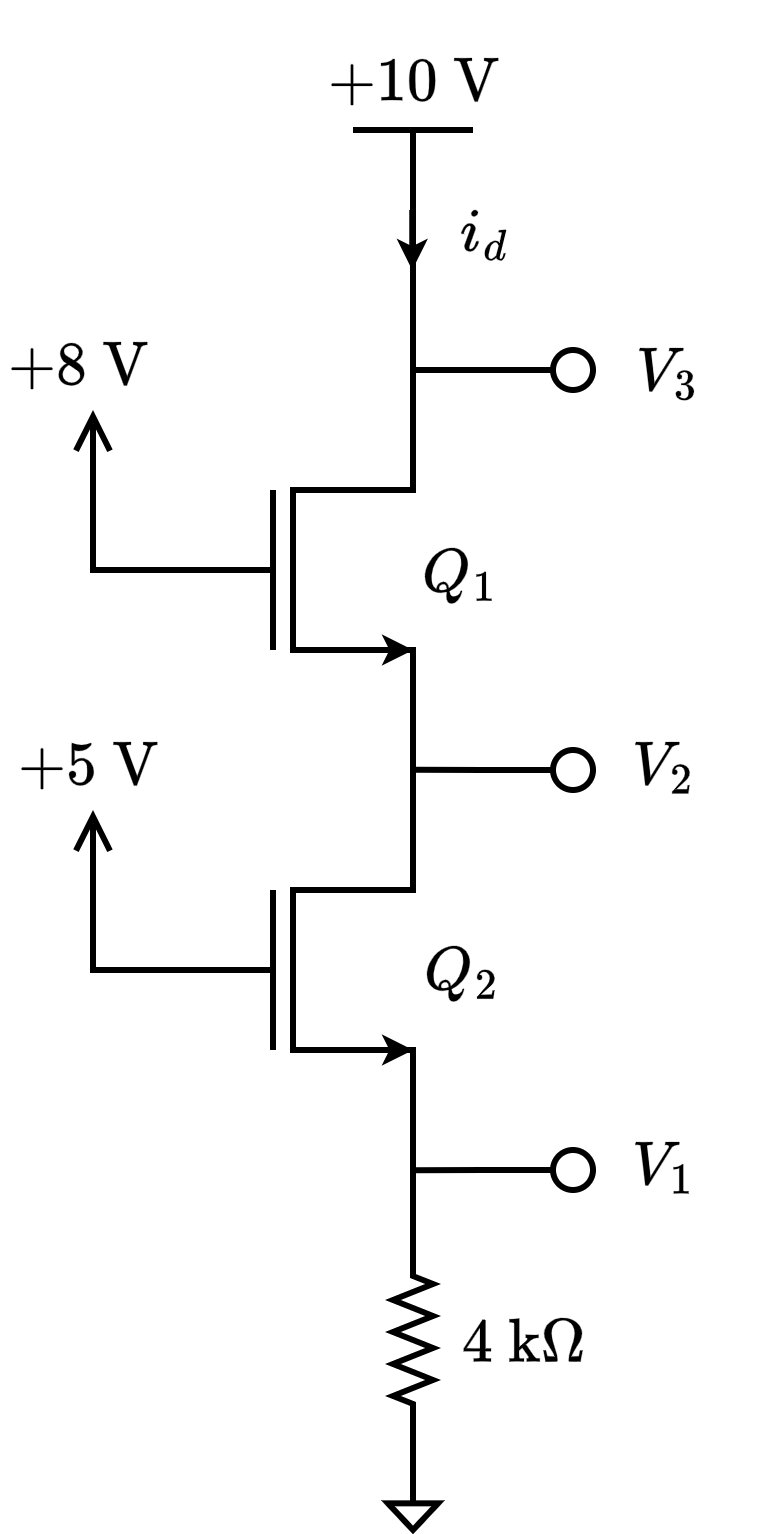
\includegraphics[height=5in]{nmos.png}
\end{center}

\begin{partquestion}{findvoltages}{What are the resulting DC bias voltages $V_{1}$, $V_{2}$, and $V_{3}$?}
\begin{answer}
Well, $V_{3}$ is immediately obvious---it is +10 V! For NMOS saturation:
\begin{align*}
    v_{DS} &\geq v_{GS} - V_{tn} \\
    v_D - v_S &\geq v_G - v_S - V_{tn} \\
    v_D &\geq v_G - V_{tn}
\end{align*}

Consider transistor $Q_{1}$, where $V_{G1} = \qty{8}{\volt}$ and $V_{D1} = \qty{10}{\volt}$. Since $10 \geq 8 - 1 = 7$, this device will be in saturation as long as it is not in cutoff, which would occur when $v_{GS1} < V_{tn}$ or equivalently when $V_{2} = v_{S1} > v_{G1} - V_{tn} = 8 - 1 = \qty{7}{\volt}$. If $Q_{1}$ is in saturation, $Q_{2}$ cannot be in cutoff, otherwise current would not flow through $Q_{1}$. Let us assume that both devices are in saturation and check for possible contradictions that arise with the analysis. Since both transistors have identical $k_{n}$ and $V_{tn}$, and for saturation $i_{D} = \frac{1}{2}k_{n}\left(V_{GS} - V_{tn} \right)^{2}$, it follows that both must have the same $V_{GS}$ if the currents are the same; that is, $V_{GS1} = V_{GS2}$. So we have the relationship:
\begin{align*}
    8 - V_2 &= 5 - V_1 \\
    V_1 &= V_2 - 3
\end{align*}
Additionally, we have:
\begin{align*}
    i_D &= \frac{1}{2} k_n (V_{GS1} - V_{tn})^2 \\
    &= \frac{1}{2} k_n (V_{G1} - V_{S1} - V_{tn})^2 \\
    &= \frac{1}{2} (5) (8 - V_2 - 1)^2 \\
    &= \frac{5}{2} (7 - V_2)^2
\end{align*}
and
\begin{align*}
    i_D &= \frac{1}{2} k_n (V_{GS2} - V_{tn})^2 \\
    &= \frac{1}{2} k_n (V_{G2} - V_{S2} - V_{tn})^2 \\
    &= \frac{1}{2} (5) (5 - V_1 - 1)^2 \\
    &= \frac{5}{2} (4 - V_1)^2
\end{align*}
so, since this must be equal to the current through the resistor, gives:
\begin{align*}
    \frac{5}{2} (4 - V_1)^2 &= \frac{V_1}{4} \\
    \frac{5}{2} (V_1^2 - 8V_1 +16) &= \frac{V_1}{4} \\
    2.5V_1^2 - 20.25V_1 + 40 &= 0
\end{align*}
which has two potential solutions $V_{1} = \qty{3.416}{\volt}$ or $V_{1} = \qty{4.684}{\volt}$. Do these work to keep $Q_2$ out of cutoff? Note the second solution would force the transistor into cutoff as $5 - 4.684 = 0.316 < V_{tn}$. What about the first? Well $5 - 3.416 = 1.58 > V_{tn}$ so it seems fine. What about $Q_1$? Using $V_1 = V_2 - 3$, we find $V_2 = 6.416$. Earlier we showed $Q_1$ would be in cutoff if $V_2 > 7$, and since $6.416 < 7$, we are in the clear!

In summary, we have found:
\begin{gather*}
V_3= \qty{10}{\volt} \\
    V_2 = \qty{6.416}{\volt} \\
    V_1 =\qty{3.416}{\volt}
\end{gather*}
Let's again show $Q_1$ is in saturation:
\begin{align*}
    V_{GS1} - V_{tn} &\overset{?}{<} V_{DS1} \\
    8 - 6.416 -1 &\overset{?}{<} 10 - 6.416 \\
    0.584 &< 3.584
\end{align*}
And now for $Q_2$:
\begin{align*}
    V_{GS2} - V_{tn} &\overset{?}{<} V_{DS2} \\
    5 - 3.416 -1 &\overset{?}{<} 6.416 - 3.416 \\
    0.584 &< 3
\end{align*}
\end{answer}
\end{partquestion}

\begin{partquestion}{findcurrent}{At these bias levels, what is the current $i_{D}$?}
\begin{answer}
We have a couple options. We can use the equation for current in saturation for either $Q_{1}$ or $Q_{2}$, or we could use Ohm's law across the resistor. Let's choose $Q_{1}$ for more practice!
\begin{align*}
    i_D &= \frac{1}{2} k_n (7 - V_2)^2 \\
    &= \frac{1}{2} (5) (7 - 6.416)^2 \\
    &= \frac{1}{2} (1.705)\\
    &= \qty{0.853}{\milli\ampere}
\end{align*}

And now with Ohm's law to confirm:
\[i_D = V_1 /\qty{4}{\kilo\ohm} = \qty{3.416}{\volt} / \qty{4}{\kilo\ohm} = \qty{0.854}{\milli\ampere}\]
The slight difference in the answers can be attributed to rounding error.
\end{answer}
\end{partquestion}

\begin{partquestion}{nowpmos}{Repeat parts (\cref{prob:seriesmosbias:findvoltages}) and (\cref{prob:seriesmosbias:findcurrent}) with this stack of PMOS devices shown below. Assume $k_p = 5\frac{\text{mA}}{V^{2}}$ and $V_{tp} = -\qty{1}{\volt}$}

\begin{center}
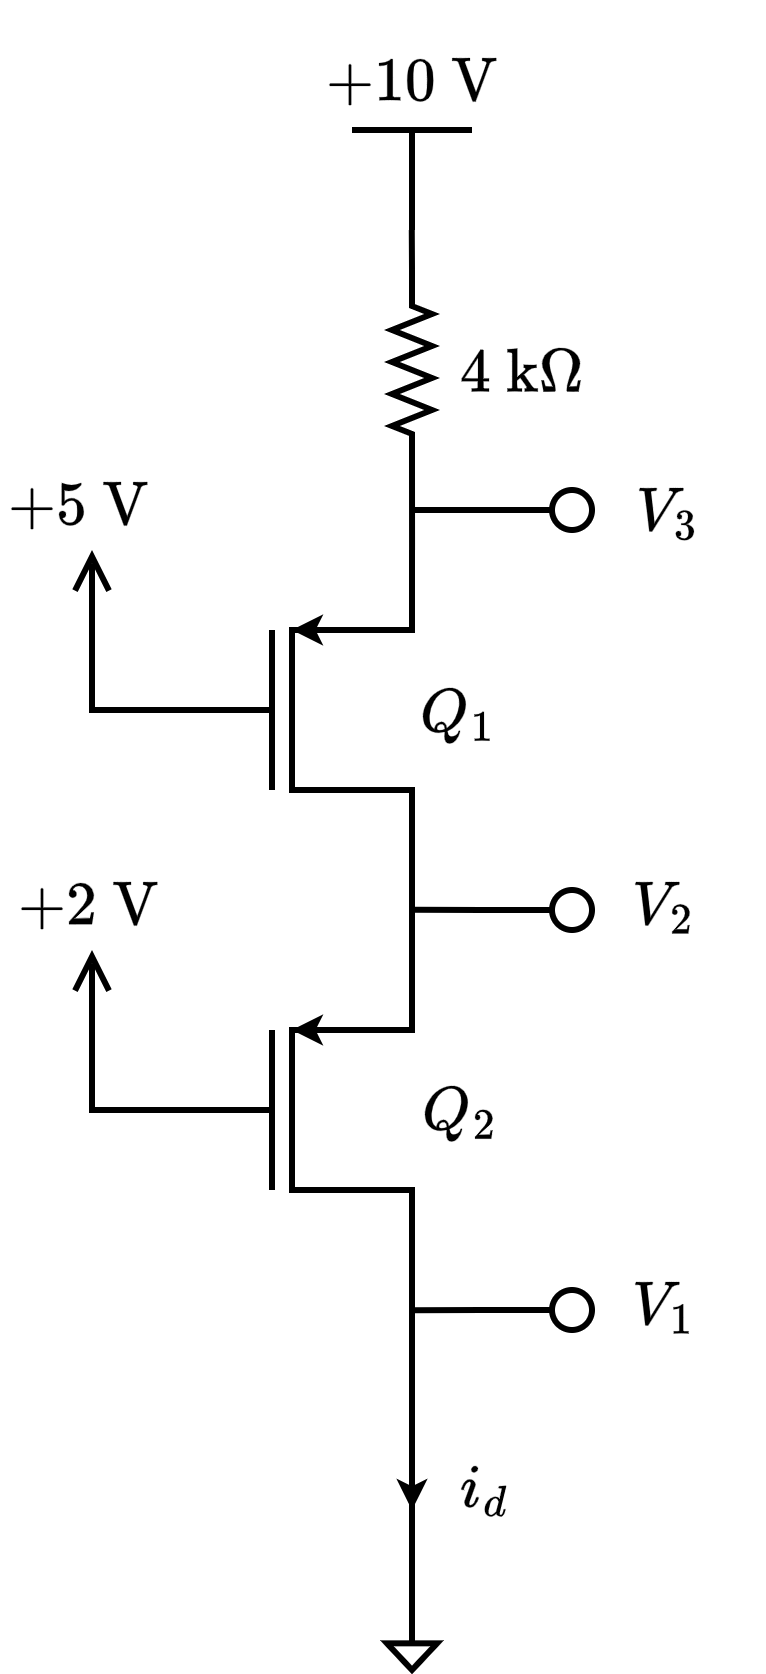
\includegraphics[height=5in]{pmos.png}
\end{center}


\begin{answer}
The quickest way to solve this is to recognize the question is complementary to the previous problem. Notice the circuit has effectively been flipped vertically. The resistor has been moved up to the 10V supply, the bias voltages have the same offsets from the 10V supply as they used to from ground, and the PMOS devices have the same transconductance and threshold voltages as the original NMOS devices. Since all these symmetries hold, we can expect the new voltages $V_{1}$, $V_2$ and $V_3$ to have the same offsets with respect to the 10V supply as the old voltages $V_1$, $V_2$ and $V_3$ had with respect to ground.
To put it mathematically:
\begin{gather*}
    V_{3,\text{pmos}} = 10V - V_{1,\text{nmos}} = \qty{6.584}{\volt}\\
    V_{2,\text{pmos}} = 10V - V_{2,\text{nmos}} = \qty{3.584}{\volt}\\
    V_{1,\text{pmos}} = 10V - V_{3,\text{nmos}} = \qty{0}{\volt}
\end{gather*}
Similarly, we would expect the drain current to be unchanged, which we can show through Ohm's law:
\[
i_d = (10 - 6.584) / 4000 = \qty{0.854}{\milli\ampere}
\]
\end{answer}
\end{partquestion}

\end{mainquestion}